
% ════════════════════════════════════════════
% 效应测算与决策解释（5.4）
% ════════════════════════════════════════════
\subsection{效应测算与决策解释}

\subsubsection{测算口径与可比性}

本部分读取回归阶段保存的最终模型 M2，固定一组代表性画像，使不同处理组之间只差一个变量。画像取 Photo、主题 1、7 月、周四、上午、粉丝规模 129,600 人；该组合的各个水平在样本中都有充足观测，避免外推到稀疏单元。付费情景只把付费标记改为 1，自然情景改为 0，其余分量保持不变。需要说明的是，粉丝规模与月份在样本中近乎一一对应，月份对粉丝规模对数的解释度达 0.9917，M2 以月份固定效应吸收规模趋势；因此画像中的粉丝规模取值用于标明情景所处的发展阶段，在样本的规模—月份对应关系下，固定月份、内容类型与时段后，处理组与对照组之间即满足“粉丝量相同”的口径。

最终模型的因变量为 log1p 曝光量，线性预测值只能解释为对数尺度上的条件均值。若直接取指数，得到的是条件几何均值，会系统性低估曝光次数的算术均值。Duan 提出的烟雾还原用残差的经验分布修正这一偏差\cite{duan1983}：
\begin{equation}
    \hat m(\boldsymbol{x})=e^{\hat\eta(\boldsymbol{x})}\hat\lambda-1,
    \qquad
    \hat\lambda=\frac{1}{n}\sum_{i=1}^{n}e^{e_i},
\end{equation}
其中 $\hat\eta(\boldsymbol{x})$ 为对数尺度预测值，$e_i$ 为训练样本残差，$\hat\lambda$ 为烟雾因子，本样本为 2.1896。区间估计采用参数模拟：从以点估计为均值、以 HC3 协方差为协方差矩阵的多元正态分布中独立抽取 1000 组系数，每组计算代表性画像与全样本的效应，取 2.5\% 与 97.5\% 分位数作为 95\% 区间。该方法同时传播多个系数的协方差，适合倍数与差值这类非线性函数。

在解读付费系数前，图\ref{fig:q4_balance}核对两组可比性。左上图把两组粉丝规模对数的提琴图、箱线与散点并排，自然组与付费组的均值分别为 11.711 与 11.715，标准化均值差仅 0.031，两个分布几乎完全重叠；右上图逐月给出付费占比与 Wilson 95\% 区间，各月在 16.0\% 至 40.0\% 之间波动，整体线 27.8\% 落在多数月份的区间内；左下与右下分别给出类型与主题构成，Photo 在两组都占 85\% 以上，主题构成的差异不超过 4.2 个百分点。唯一可见的差异是付费组 Video 占 2.9\%、自然组仅 0.8\%，但 Video 总共只有 7 条，且回归已用类型哑变量吸收其影响。由此可见，两组在可观测特征上接近，后文约 40\% 的提升不太可能由粉丝规模或内容构成差异解释。

\begin{figure}[ht]
  \centering
  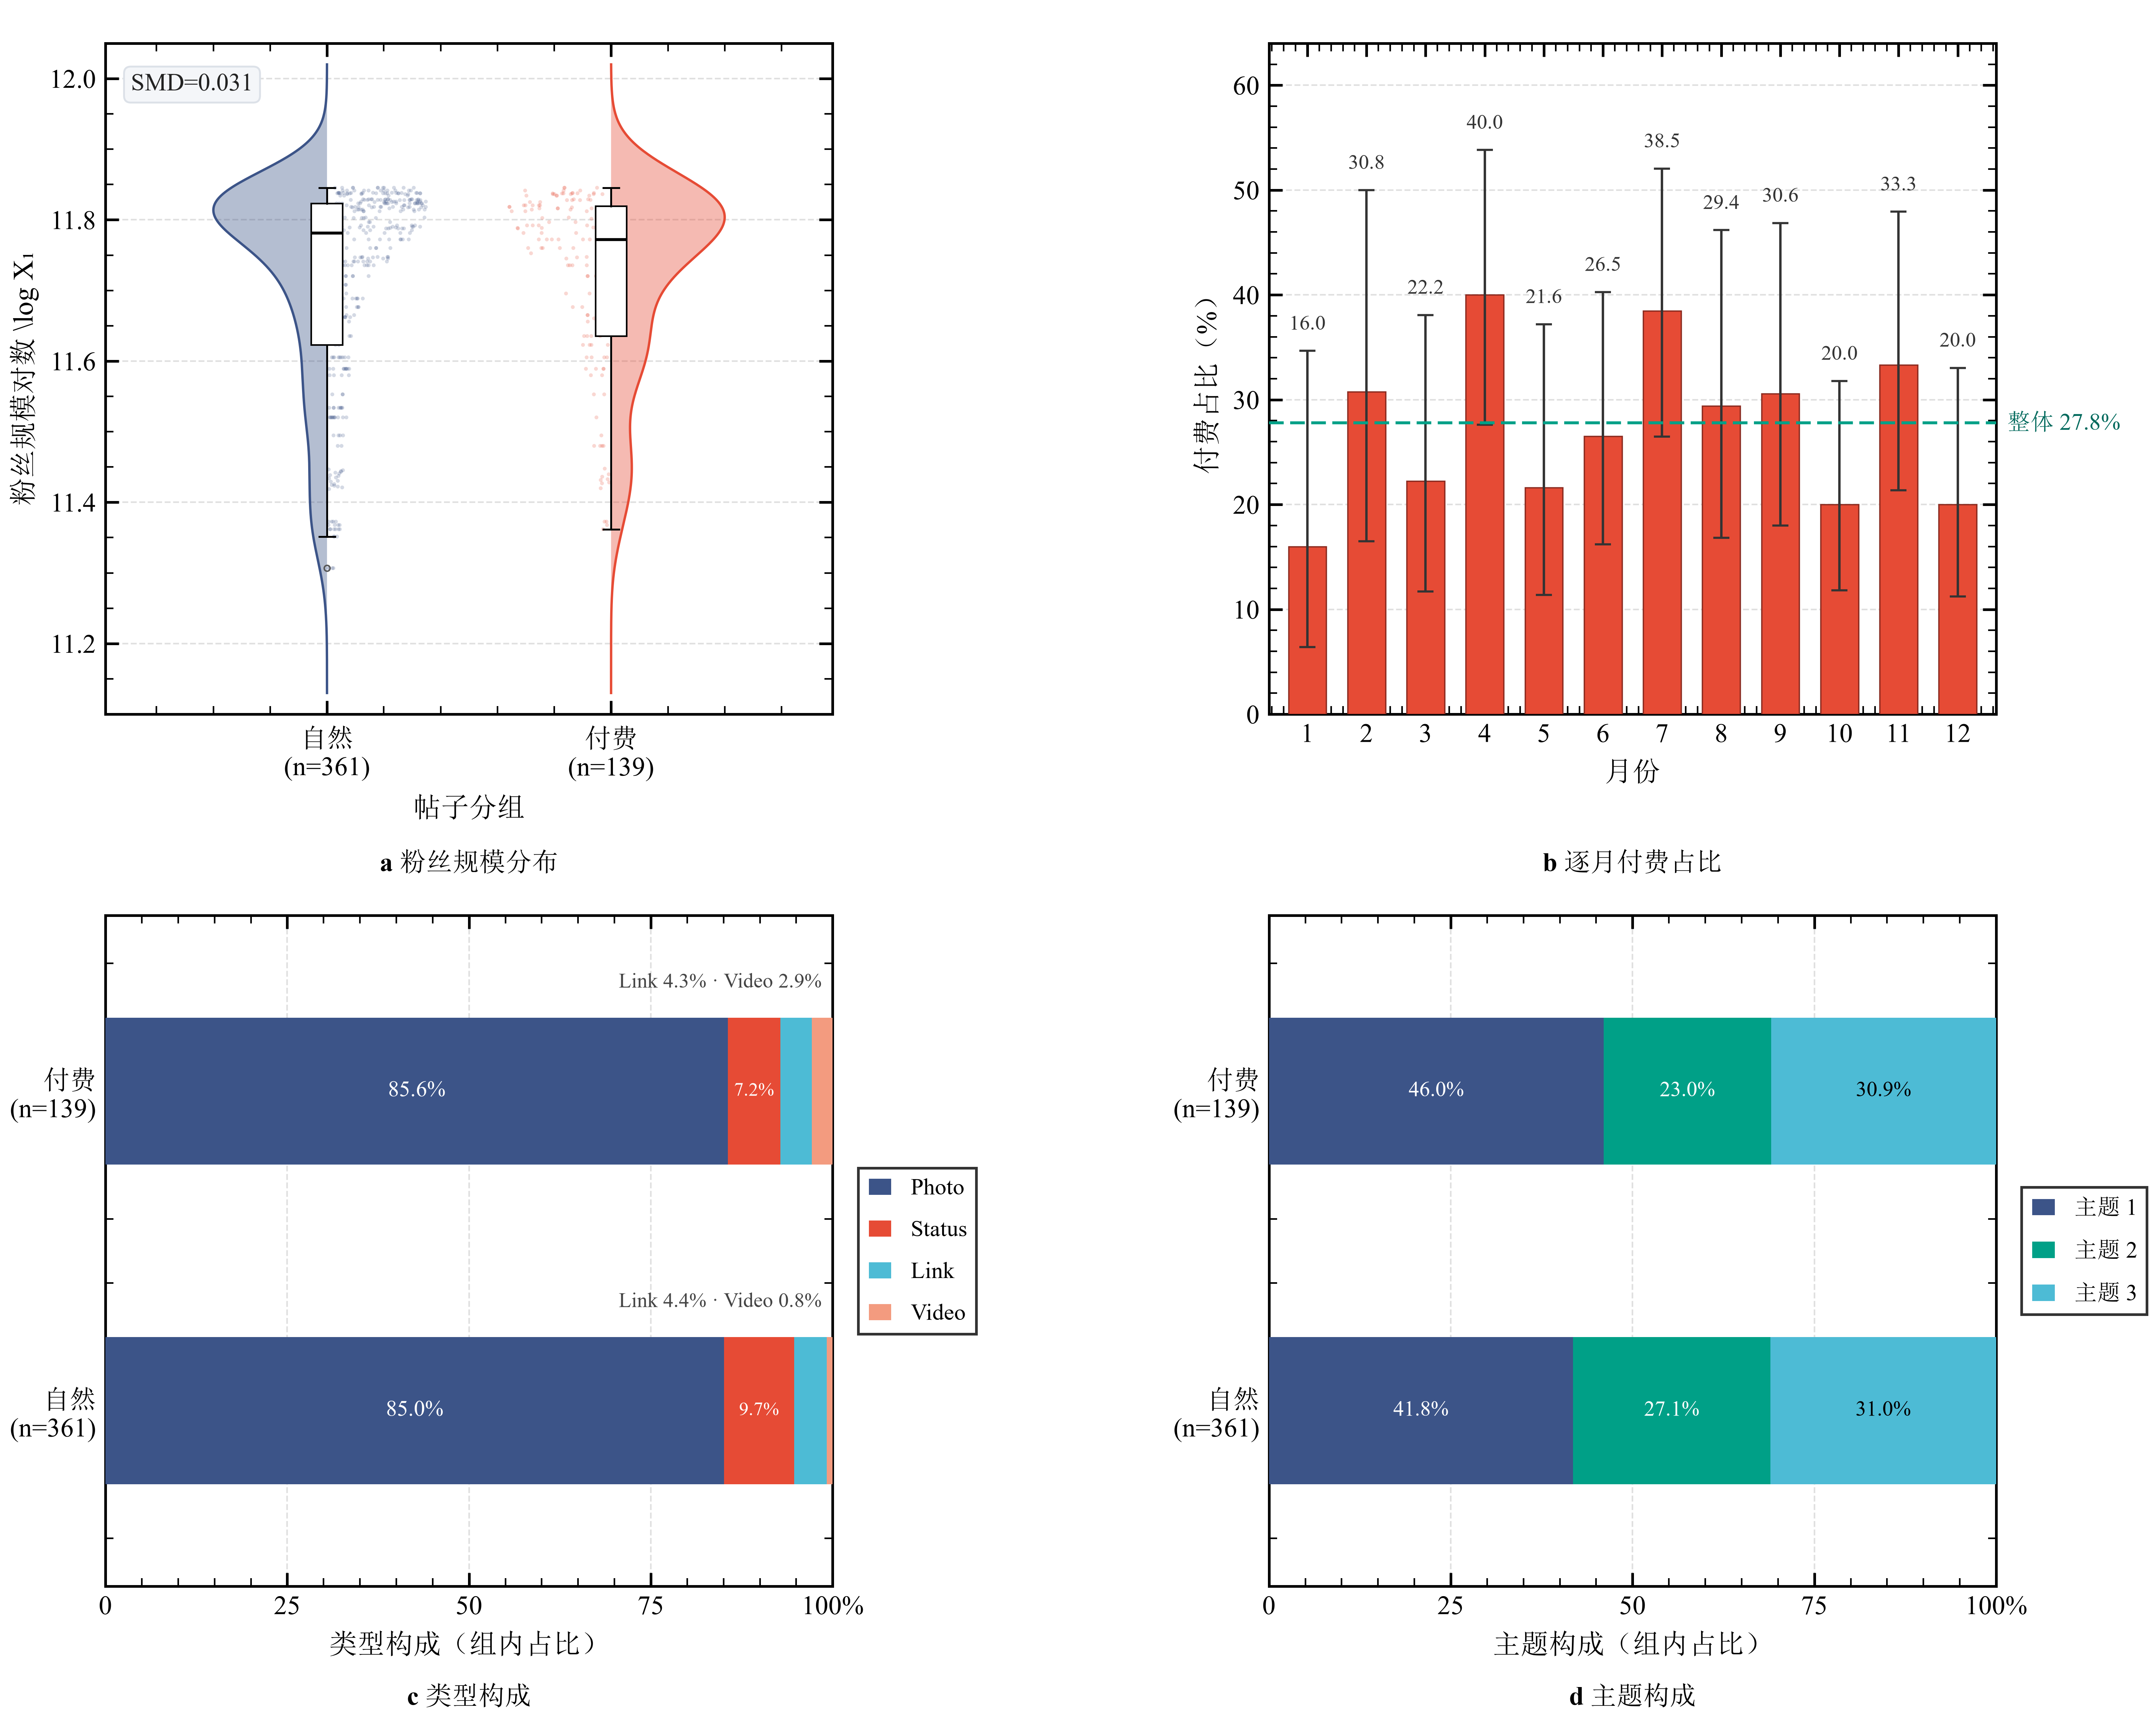
\includegraphics[width=0.70\textwidth]{../求解/临时产物/补充图3_付费可比性.png}
  \caption{付费组与自然组的可比性}
  \label{fig:q4_balance}
\end{figure}

\subsubsection{付费、类型与主题效应}

付费效应的点估计为 0.3374，HC3 标准误 0.1195，95\% 置信区间 0.1025 至 0.5723，对应净提升 40.13\%、区间 10.80\% 至 77.24\%。在代表性画像上，自然帖子的调整预测曝光为 40,221 次，付费帖子为 56,364 次，差值 16,142 次，区间 4,543 至 33,467 次，倍数 1.401、区间 1.104 至 1.753。全样本反事实的平均处理效应为 10,907 次，区间 3,138 至 20,195 次，倍数同样为 1.401。作为未调整的对照，完整案例中付费组的中位曝光为 12,060 次、自然组为 8,443 次，中位数比 1.429；填补后自然组为 361 条、中位 8,387 次，比值 1.438，与调整后的 1.401 非常接近，说明付费的正向差异不是由内容类型或发布时机的构成差异造成的。

图\ref{fig:q4_pred}把付费、类型与主题的调整预测放在同一张图中。左上图显示付费与自然的区间在曝光尺度上有重叠，但点估计的差值明确为正；右上图按类型排列，Video 的点估计远高于其他三类，区间也最宽；左下图显示主题 2 的调整预测最低（2.49 万次），主题 1 最高（4.02 万次），主题 3 为 2.94 万次；右下图按付费与类型分组给出观测中位数，Photo、Status、Link 三条连线向上，Video 因仅 7 条且付费组只有 4 条，中位数由 5.70 万次降至 5.08 万次。交互检验的 $p$ 值为 0.530，不能据此认为付费效应在不同内容类型之间存在显著差异，主效应模型已经足够。

\begin{figure}[ht]
  \centering
  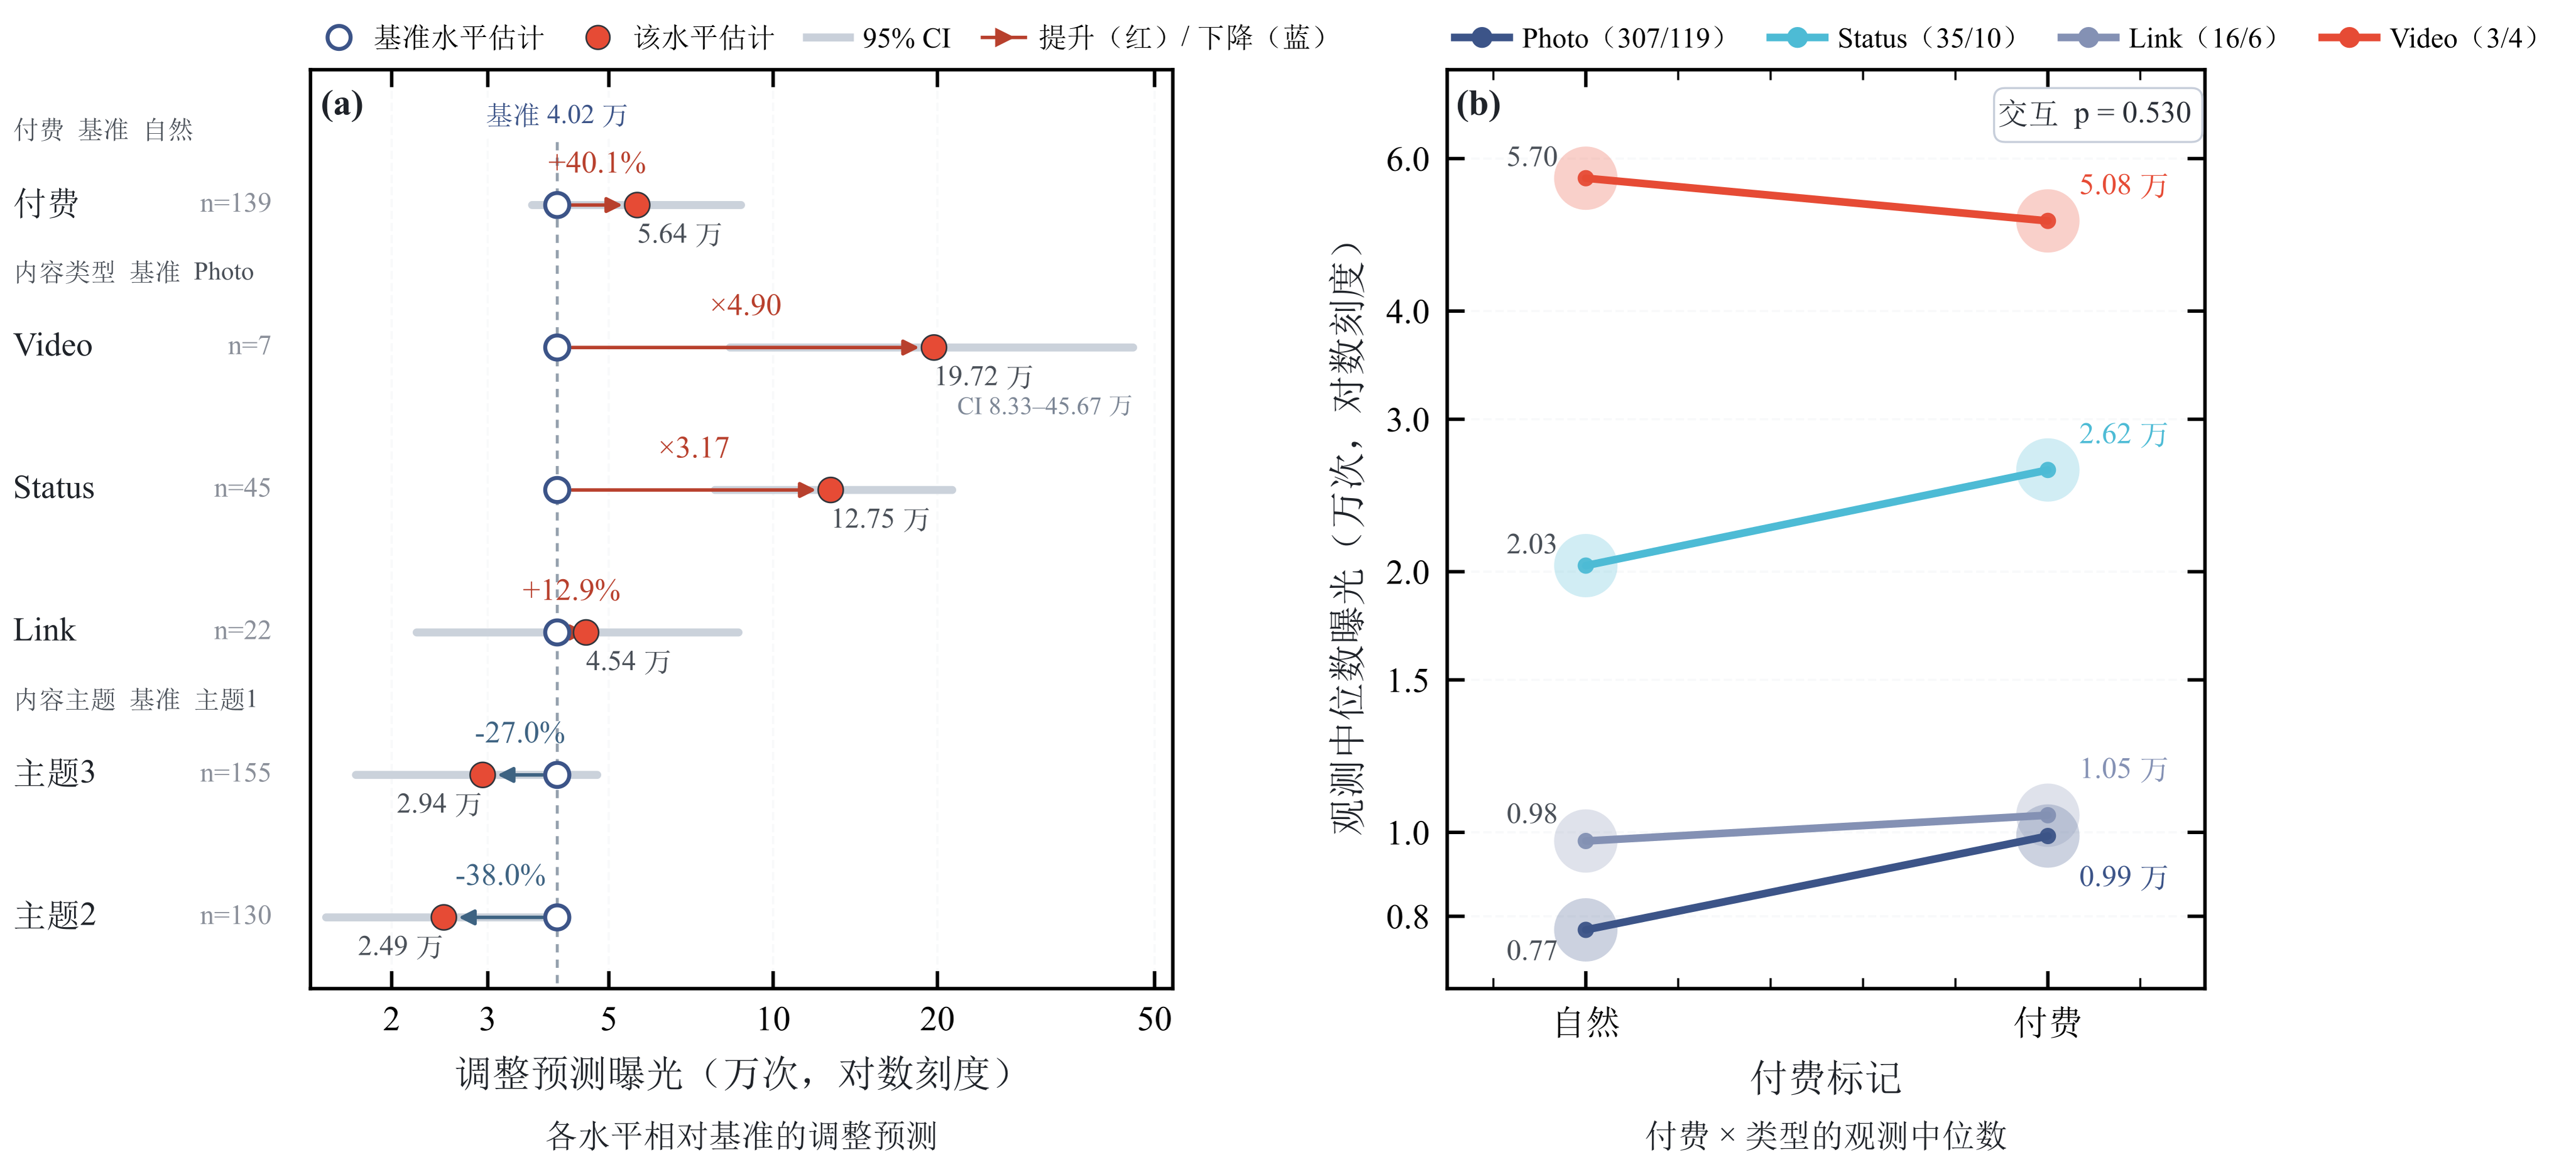
\includegraphics[width=0.75\textwidth]{../求解/问题四/结果/图11_调整预测效应.png}
  \caption{付费、内容类型与内容主题的调整预测曝光}
  \label{fig:q4_pred}
\end{figure}

内容类型与内容主题的对比如表\ref{tab:q4_effect}所示。以 Photo 为参照，Video 的系数为 1.5896、$p$ 值 0.0001，折算为 4.90 倍，区间 2.23 至 10.79；Status 的系数为 1.1538、$p$ 值小于 0.001，折算为 3.17 倍，区间 2.49 至 4.04；Link 的系数为 0.1215、$p$ 值 0.643，折算为 1.13 倍，区间 0.68 至 1.89，与 Photo 无显著差异。在代表性画像上，Video 的调整预测曝光为 197,157 次，比 Photo 的 40,221 次多出约 15.7 万次；Status 为 127,511 次，Link 为 45,420 次。Video 的倍数最高，但其区间上限约为下限的 4.8 倍，且样本只有 7 条，解读时应把它理解为“方向明确、幅度不确定”的信号，而不是精确的投放回报。

内容主题的联合与两两结果同样列在表\ref{tab:q4_effect}。联合 Wald 统计量为 12.6783、自由度 2、$p$ 值 0.0018，拒绝“两个主题哑变量同时为零”的原假设，说明主题整体对曝光有显著影响。相对主题 1，主题 2 的系数为 $-0.4784$、折算 0.620 倍，区间 0.475 至 0.808；主题 3 的系数为 $-0.3147$、折算 0.730 倍，区间 0.561 至 0.950。两者都显著低于主题 1，且主题 2 的点估计更低。但主题 2 与主题 3 的直接差异为 $-0.1638$、$p$ 值 0.186、倍数 0.849，区间 0.666 至 1.082，在 5\% 水平不显著，不能据此断言主题 2 一定劣于主题 3。

\begin{longtable}{>{\centering\arraybackslash}p{0.19\textwidth}>{\centering\arraybackslash}p{0.085\textwidth}>{\centering\arraybackslash}p{0.085\textwidth}>{\centering\arraybackslash}p{0.08\textwidth}>{\centering\arraybackslash}p{0.07\textwidth}>{\centering\arraybackslash}p{0.07\textwidth}>{\centering\arraybackslash}p{0.07\textwidth}>{\centering\arraybackslash}p{0.07\textwidth}}
  \caption{内容类型与内容主题效应}
  \label{tab:q4_effect} \\
  \toprule
  对比 & 系数或\newline 统计量 & 标准误 & $p$ 值 & 倍数 & 倍数\newline 下限 & 倍数\newline 上限 & 处理组\newline 曝光 \\
  \midrule
  \endfirsthead
  \caption{内容类型与内容主题效应（续）} \\
  \toprule
  对比 & 系数或\newline 统计量 & 标准误 & $p$ 值 & 倍数 & 倍数\newline 下限 & 倍数\newline 上限 & 处理组\newline 曝光 \\
  \midrule
  \endhead
  \bottomrule
  \endfoot
  Video 对 Photo & 1.590 & 0.402 & 0.0001 & 4.902 & 2.226 & 10.793 & 197,157 \\
  Status 对 Photo & 1.154 & 0.124 & $<$0.001 & 3.170 & 2.487 & 4.041 & 127,511 \\
  Link 对 Photo & 0.122 & 0.262 & 0.643 & 1.129 & 0.675 & 1.889 & 45,420 \\
  主题联合 Wald & 12.678 & — & 0.0018 & — & — & — & — \\
  主题 2 对主题 1 & $-0.478$ & 0.135 & $<$0.001 & 0.620 & 0.475 & 0.808 & 24,927 \\
  主题 3 对主题 1 & $-0.315$ & 0.134 & 0.019 & 0.730 & 0.561 & 0.950 & 29,363 \\
  主题 2 对主题 3 & $-0.164$ & 0.124 & 0.186 & 0.849 & 0.666 & 1.082 & — \\
\end{longtable}

\subsubsection{稳健性与异质性}

表\ref{tab:q4_robust}汇总六种设定下的付费与视频效应。付费提升在 M1 至 M4 中为 40.09\% 至 49.65\%，Huber 回归为 37.44\%，Gamma 模型为 44.84\%，全部在 1\% 水平显著；Video 倍数在 3.52 至 5.41 之间，同样全部显著。M3 与 M4 因未使用月份固定效应，付费系数略高，说明月份控制吸收了一部分与付费相关的季节差异；Gamma 模型的 Video 倍数最低，反映其对右偏分布的拟合更保守。六种设定的方向一致、区间都不跨过 0 或 1，可以认为结论不依赖单一模型设定。

\begin{longtable}{>{\centering\arraybackslash}p{0.19\textwidth}>{\centering\arraybackslash}p{0.10\textwidth}>{\centering\arraybackslash}p{0.09\textwidth}>{\centering\arraybackslash}p{0.10\textwidth}>{\centering\arraybackslash}p{0.10\textwidth}>{\centering\arraybackslash}p{0.09\textwidth}>{\centering\arraybackslash}p{0.09\textwidth}}
  \caption{六种设定下的付费与视频效应}
  \label{tab:q4_robust} \\
  \toprule
  设定 & 付费系数 & 付费 $p$ 值 & 付费提升\newline （\%） & Video\newline 系数 & Video\newline $p$ 值 & Video\newline 倍数 \\
  \midrule
  \endfirsthead
  \caption{六种设定下的付费与视频效应（续）} \\
  \toprule
  设定 & 付费系数 & 付费 $p$ 值 & 付费提升\newline （\%） & Video\newline 系数 & Video\newline $p$ 值 & Video\newline 倍数 \\
  \midrule
  \endhead
  \bottomrule
  \endfoot
  M1 全模型 & 0.337 & 0.005 & 40.09 & 1.588 & $<$0.001 & 4.894 \\
  M2 月份固定效应 & 0.337 & 0.005 & 40.13 & 1.590 & $<$0.001 & 4.902 \\
  M3 仅 $\log X_1$ & 0.403 & 0.001 & 49.65 & 1.658 & $<$0.001 & 5.250 \\
  M4 线性月份 & 0.386 & 0.002 & 47.14 & 1.688 & $<$0.001 & 5.408 \\
  Huber 稳健回归 & 0.318 & 0.001 & 37.44 & 1.683 & $<$0.001 & 5.384 \\
  Gamma 广义线性模型 & 0.371 & 0.010 & 44.84 & 1.258 & 0.001 & 3.518 \\
\end{longtable}

\begin{figure}[ht]
  \centering
  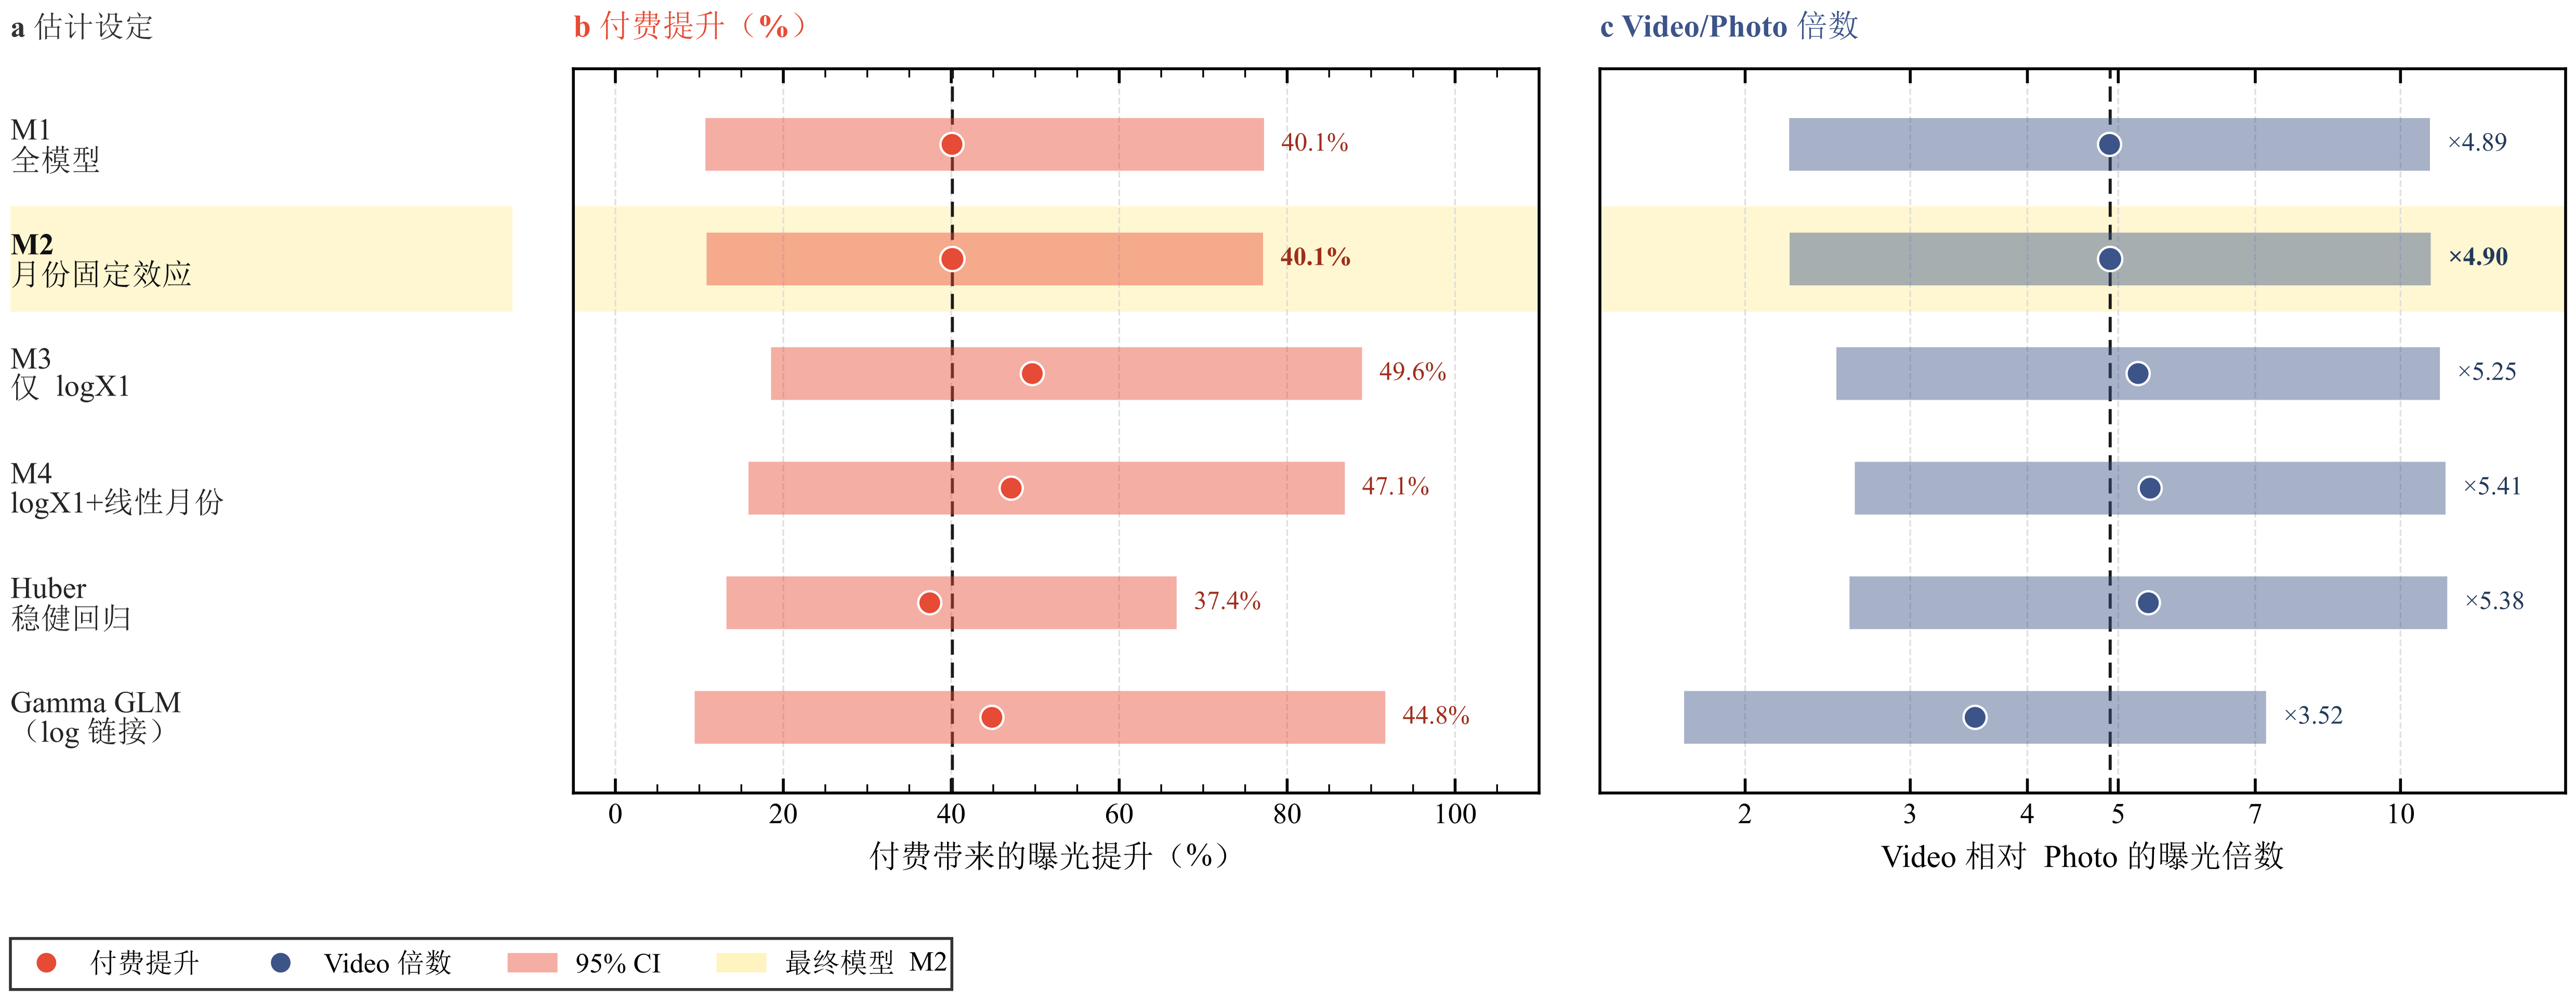
\includegraphics[width=0.75\textwidth]{../求解/问题四/结果/图12_效应稳健性.png}
  \caption{付费与视频效应在六种设定下的稳健性}
  \label{fig:q4_robust}
\end{figure}

图\ref{fig:q4_matrix}进一步把 7 个主效应在 6 种设定下的系数画成矩阵，按行归一化着色并标注显著性。付费、Video、Status、主题 2、主题 3 与时段凌晨的方向在所有设定下一致；Link 在所有设定下都不显著，Gamma 模型中甚至反号，因此不能把 Link 的相对曝光差异当作稳定结论。矩阵还显示，主题 2 的负向系数在 Gamma 模型中最强（$-0.848$），主题 3 在 M3 中减弱为不显著（$-0.236$），说明主题效应的大小对分布假设有一定敏感，但方向没有反转。

\begin{figure}[ht]
  \centering
  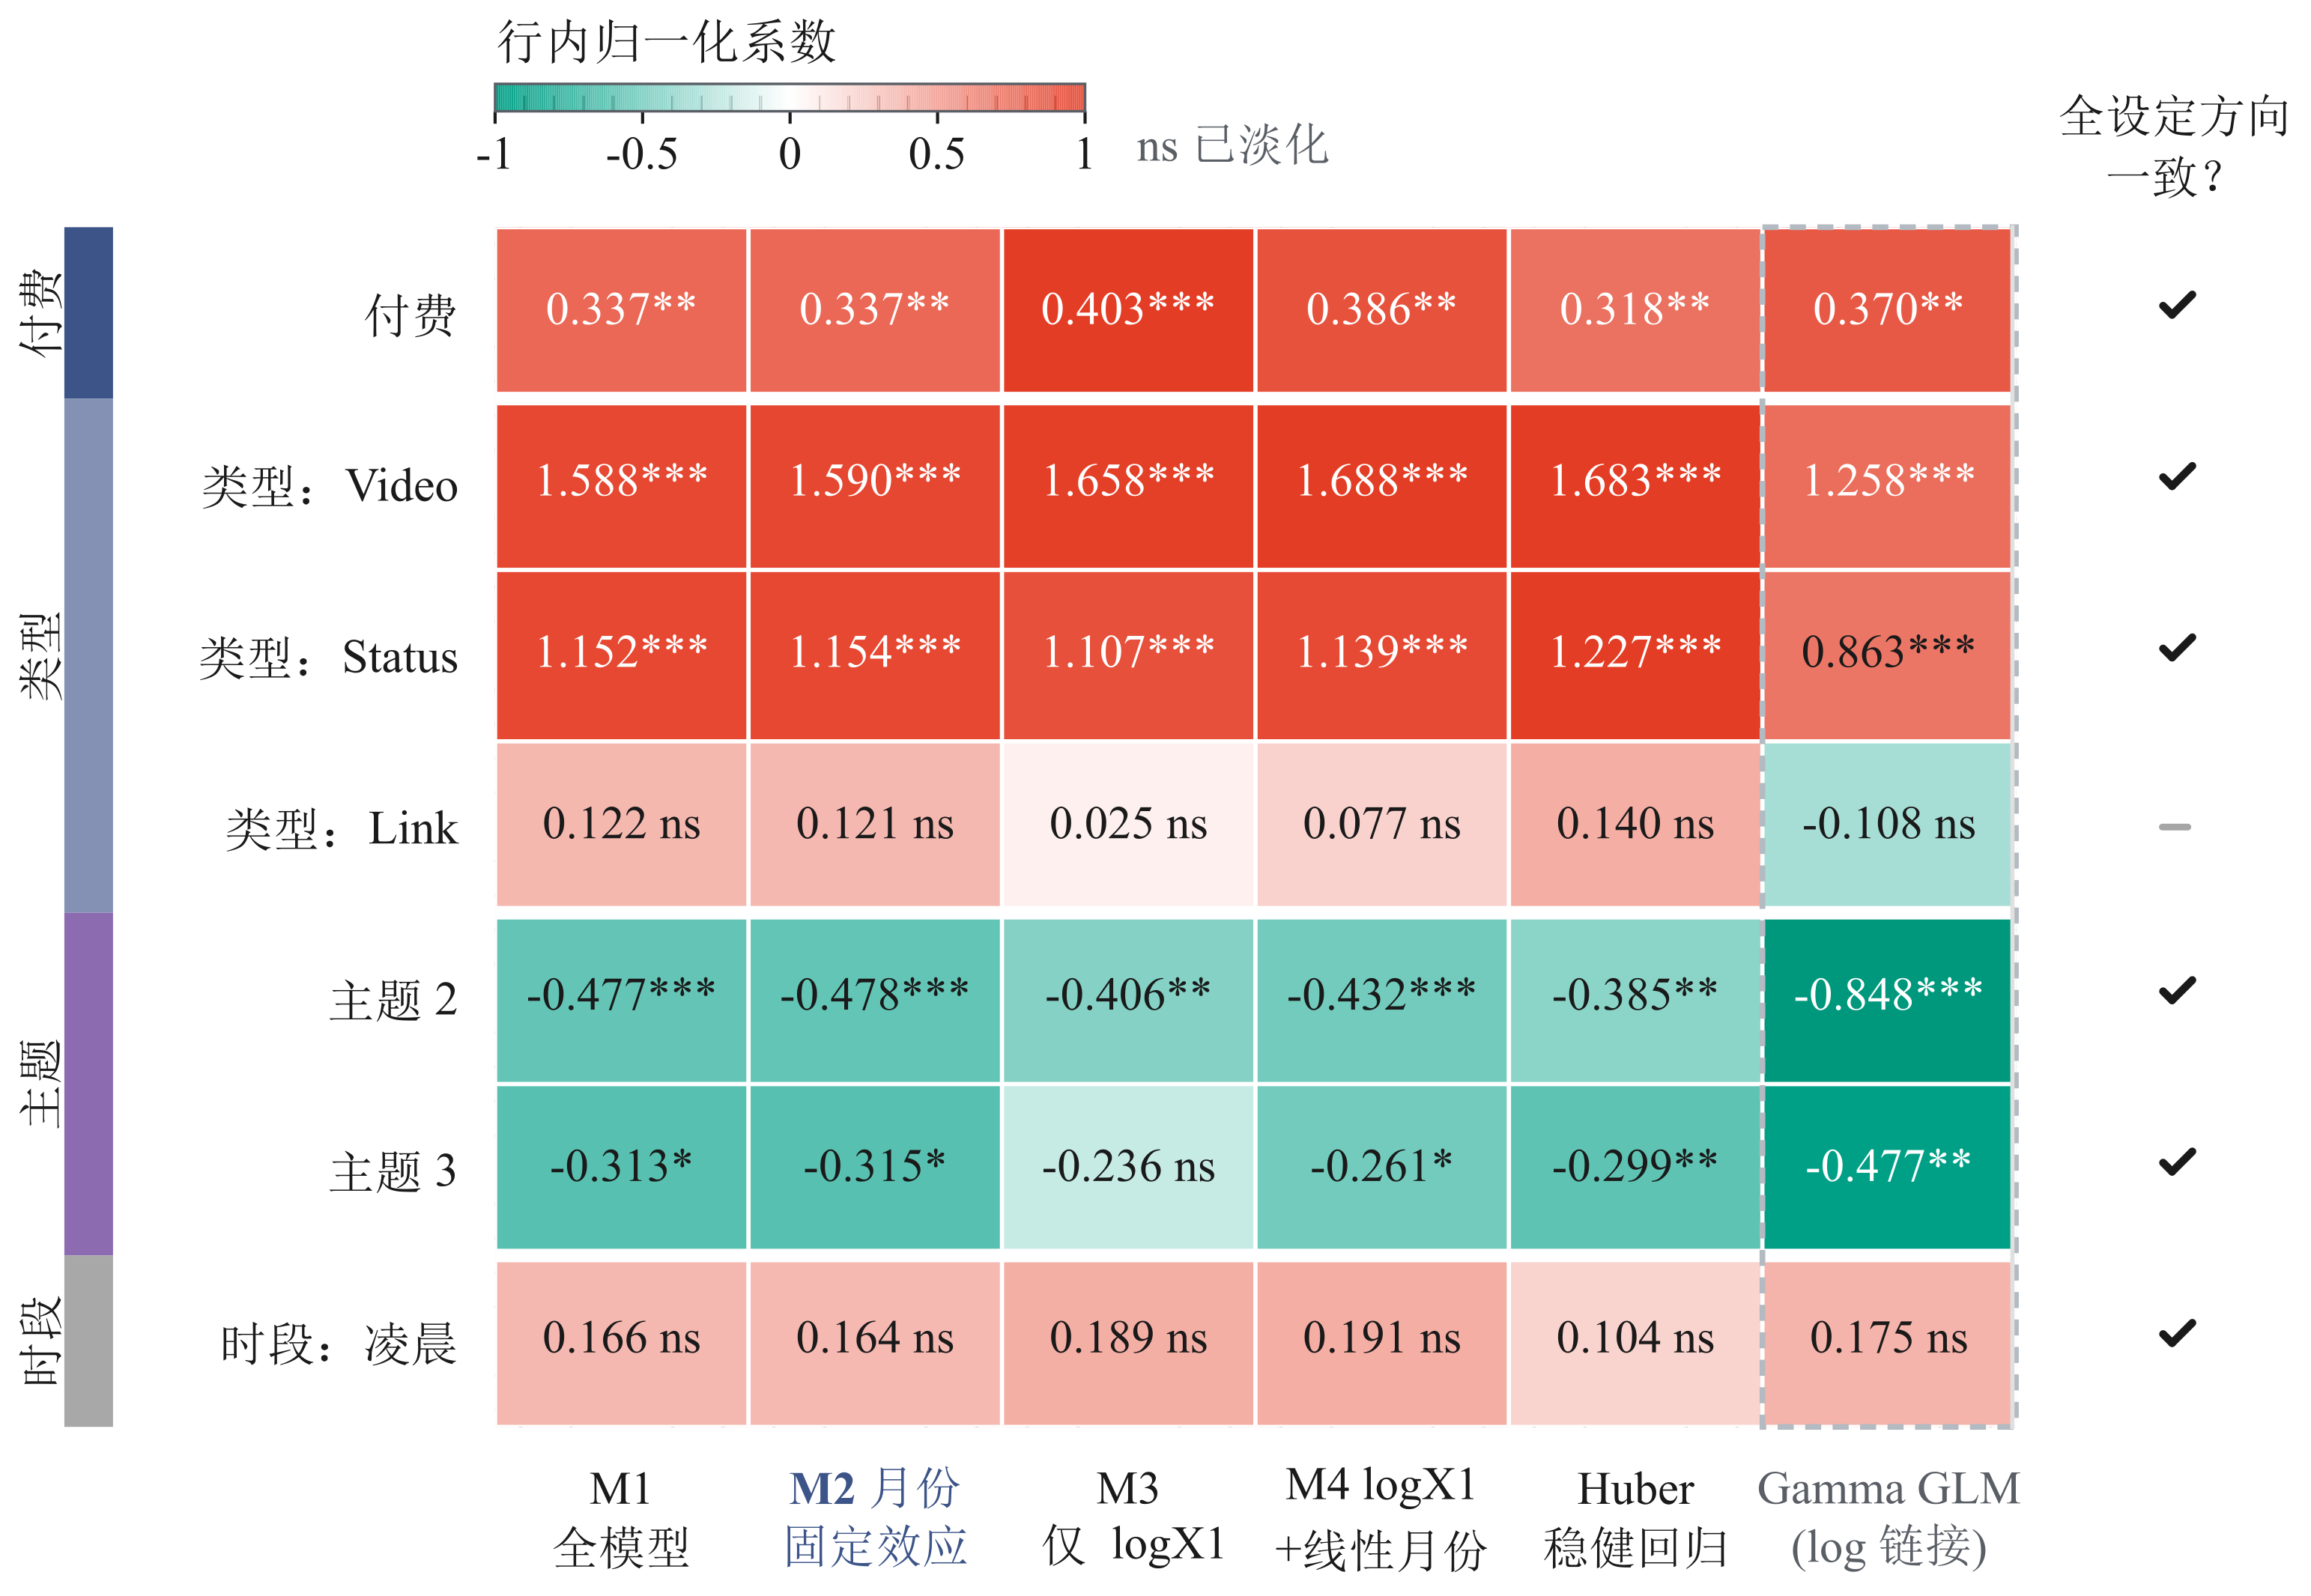
\includegraphics[width=0.70\textwidth]{../求解/问题四/结果/图16_系数稳健性矩阵.png}
  \caption{七个主效应在六种设定下的系数稳健性矩阵}
  \label{fig:q4_matrix}
\end{figure}

最后检验付费效应是否随内容特征变化。图\ref{fig:q4_het}按全样本、帖子类型、内容主题与发布时段分组，报告各组内的付费系数与交互联合检验的 $P$ 值。类型组的组内 $P$ 为 0.531，时段组为 0.474，均未拒绝“付费效应不随该维度变化”的原假设；主题组的组内 $P$ 为 0.036，在 5\% 水平显著。具体看，主题 1 的付费系数为 0.57（95\% 区间 0.15 至 0.99，$p=0.008$），主题 2 为 0.43（区间 $-0.01$ 至 0.86，$p=0.056$），主题 3 仅为 0.02（区间 $-0.40$ 至 0.45，$p=0.911$）。这说明付费投放的增量主要集中在主题 1，主题 2 处于边缘显著，主题 3 几乎看不到付费效果。若改用互斥子样本的系数 $Q$ 检验，主题组 $p$ 值为 0.172，说明该异质性证据对检验口径有一定敏感性；本报告以与图\ref{fig:q4_pred}同口径的交互联合检验为主，把主题异质性作为定向投放的参考，而不是强因果结论。

\begin{figure}[ht]
  \centering
  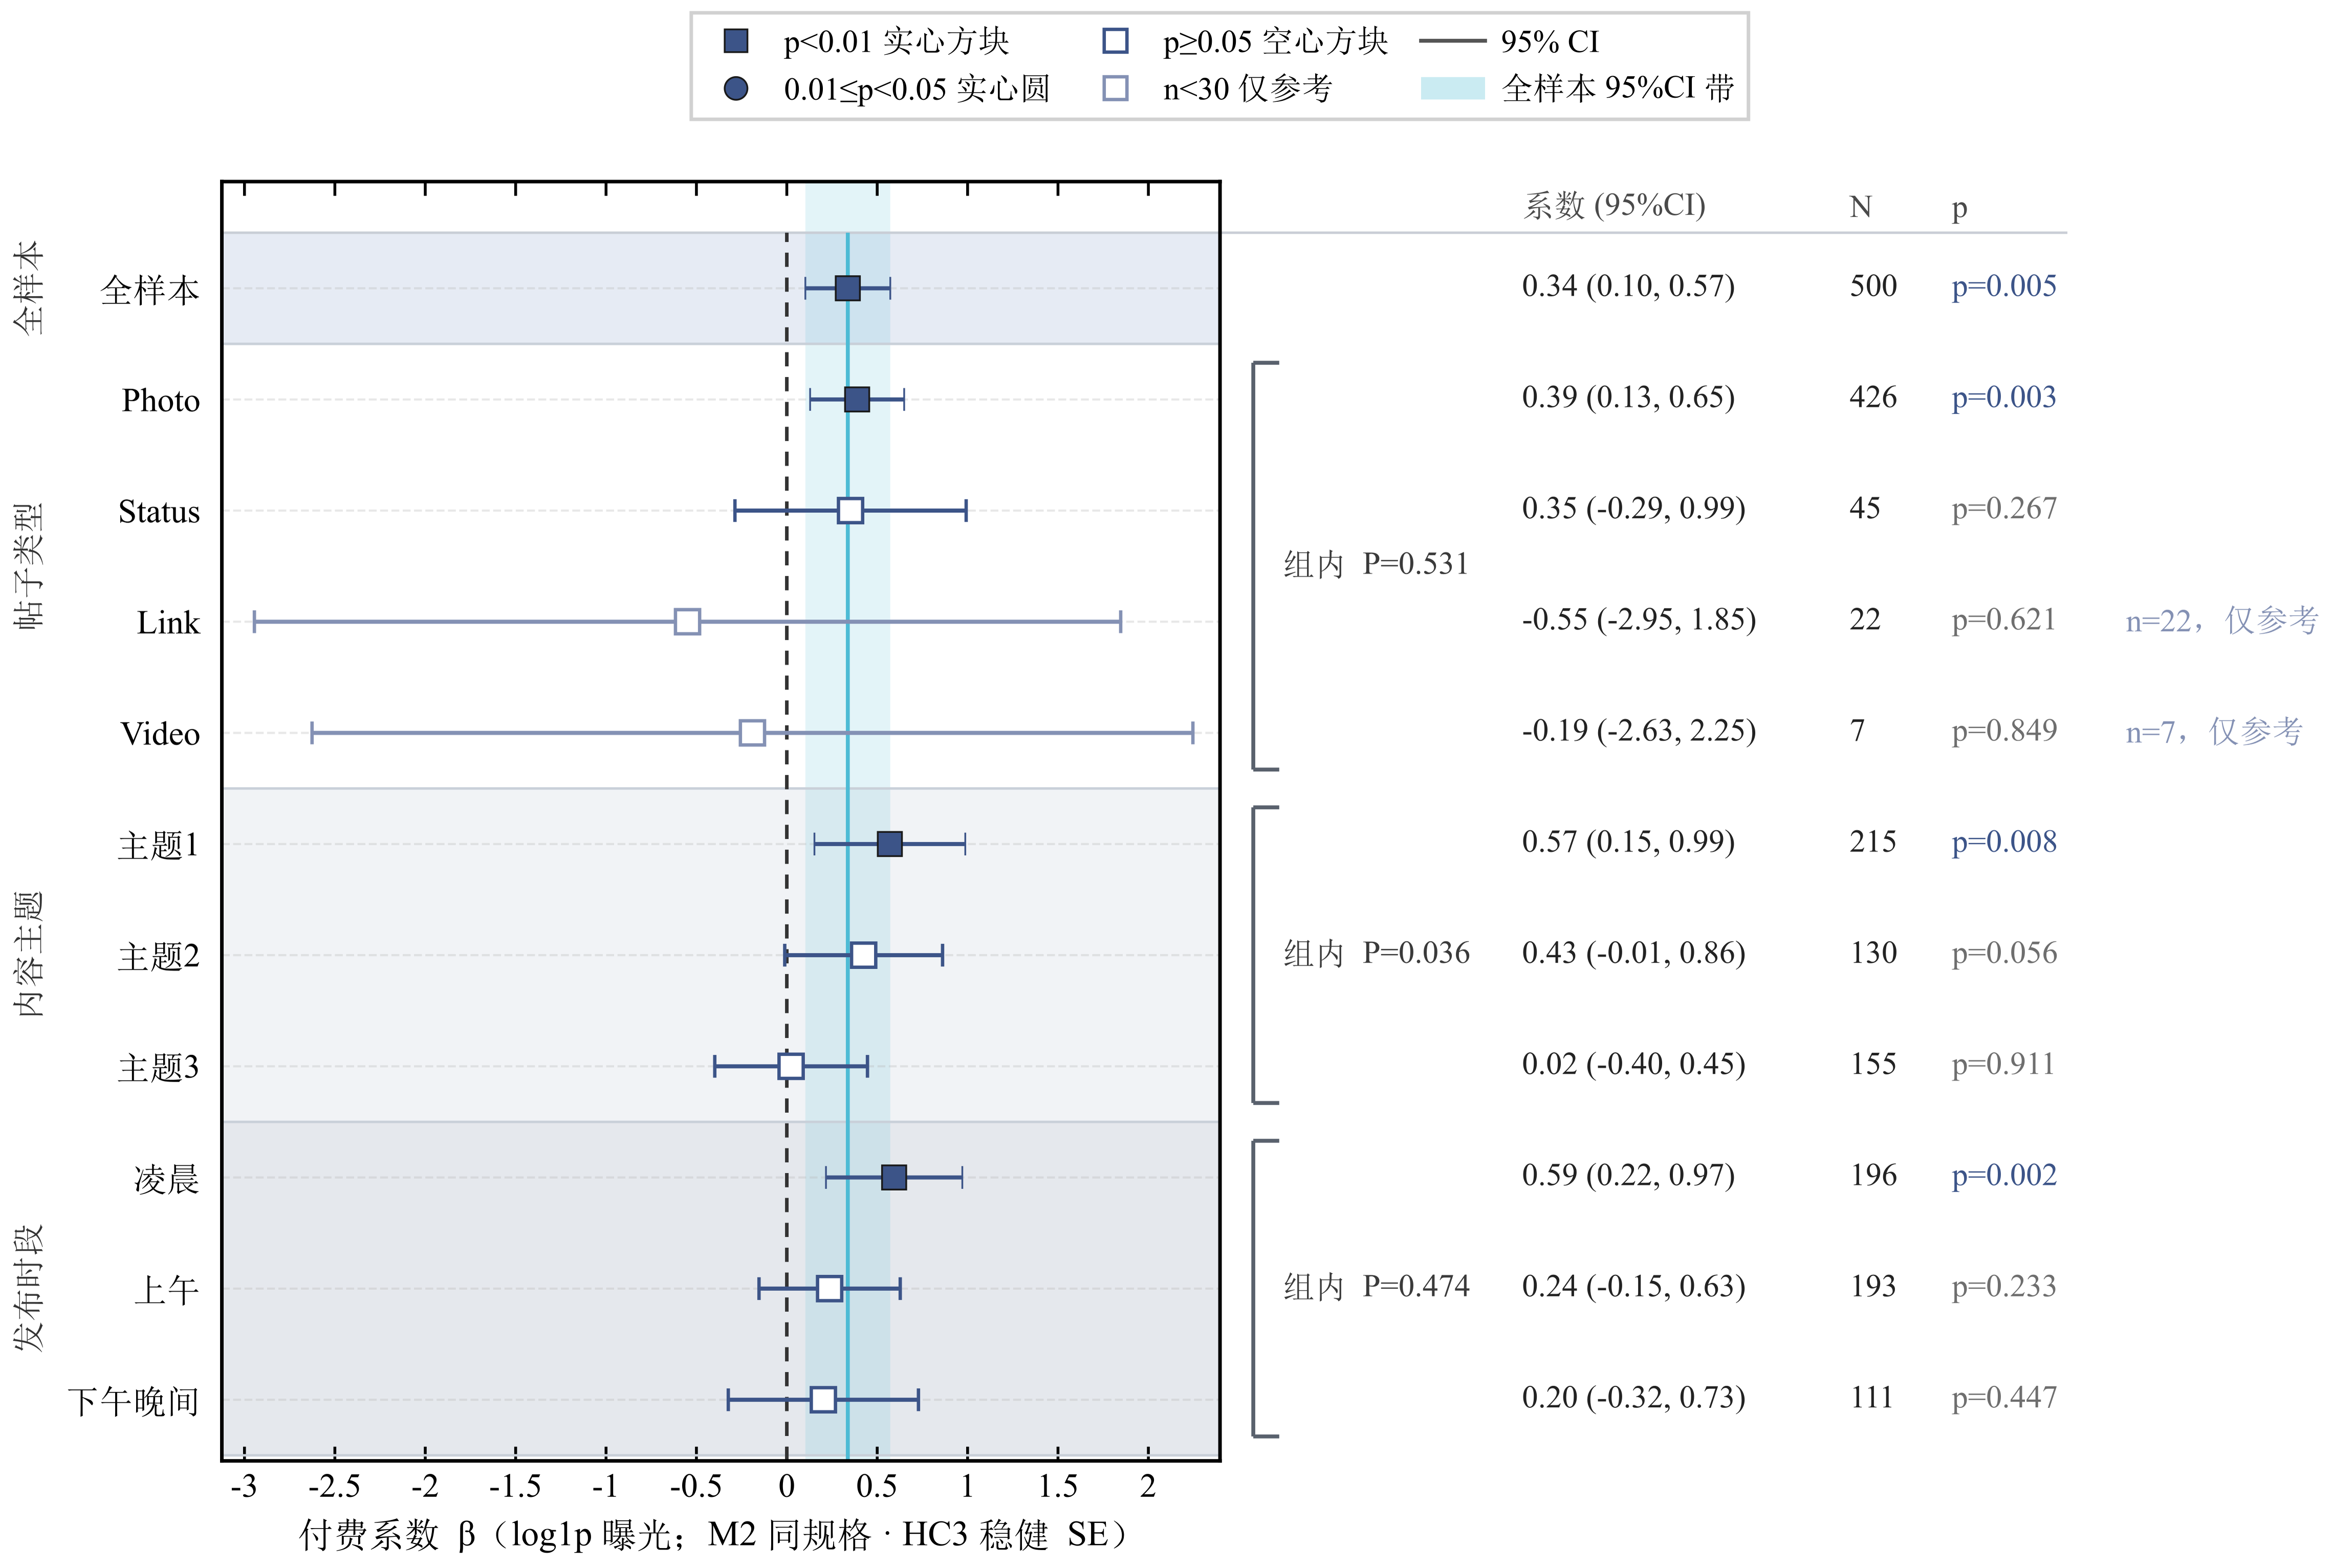
\includegraphics[width=0.70\textwidth]{../求解/问题四/结果/图17_付费效应异质性森林.png}
  \caption{付费效应在类型、主题与时段分组下的异质性}
  \label{fig:q4_het}
\end{figure}

综合以上结果，付费平均带来约 40\% 的曝光提升，代表性画像上约为 1.6 万次增量；视频相对图片约为 4.9 倍，方向明确但精度受 7 条样本限制；状态类型约为 3.2 倍，链接类型与图片无显著差异；内容主题整体显著，主题 2 与主题 3 都低于主题 1，但两者之间差异不显著。付费效应在主题维度存在异质性，主题 1 的增量最大，主题 3 接近于零。上述结论在六种模型设定下保持一致，可作为品牌主页内容编排与付费投放的参考。
